\section{Word representations} \label{bgemb} 

The first step in using neural models for text is to map the words in the vocabulary to \textit{dense vectors} of real numbers.
These vectors are somewhat similar to \textit{sparse vectors} used in distributional semantics, where they represent meaning by capturing similarities between lexical units based on their distributional properties \citep{baroni-etal-2014-dont,baroni-lenci-2010-distributional}.
The context of the lexical unit is commonly used for the computation of dense and sparse embeddings.
The intuition is that since similar words appear in similar contexts, they end up with similar embeddings \citep{firth1957synopsis}.
Computation of dense vectors is often a by-product of solving a natural language processing task such as language modeling or translation. 

Word representations can be categorized into two groups \citep{Wang2019UsingDE}: \textit{static embeddings} where a fixed vector is learned for each word in the vocabulary, and \textit{dynamic embeddings} where vectors are dynamically calculated for each sentence. 
In the next sections, we discuss different approaches in each category.

\subsection{Static embeddings}  \label{bgembstatic} 

Traditional word embedding techniques learn a global and static word embedding for every word in the vocabulary. 
\citet{mikolov2013efficient} proposed two models for learning word representations: continuous Skipgram and continuous bag-of-words (CBOW).
Both models use a feed-forward neural network architecture with the objective of modeling language, illustrated in Figure~\ref{bgsgcbowfig}.
This architecture does not include any non-linearity. 
\begin{figure}
\centering
\begin{subfigure}[t]{.45\textwidth}
  \centering
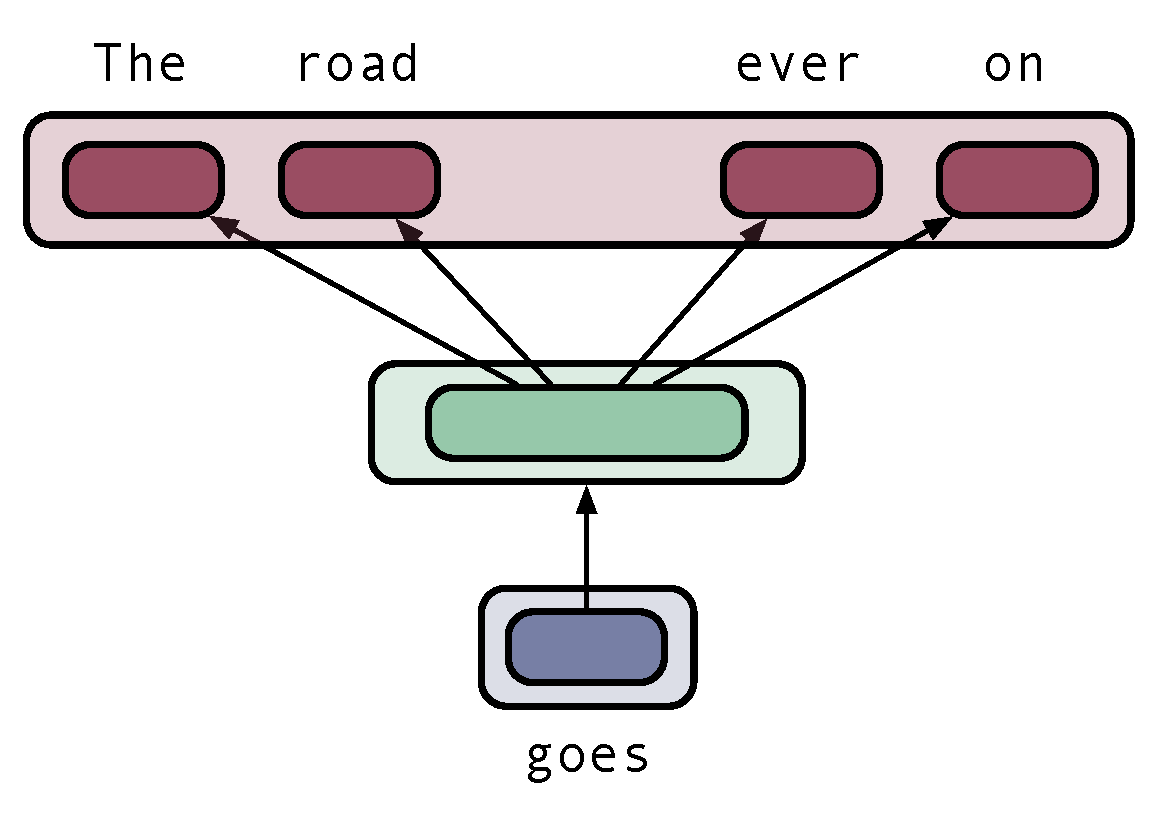
\includegraphics[width=0.8\linewidth]{02-background/figs/skipgram.pdf}
\caption{Skipgram model}
\label{bgsgfig}
\end{subfigure}%
\begin{subfigure}[t]{.45\textwidth}
  \centering
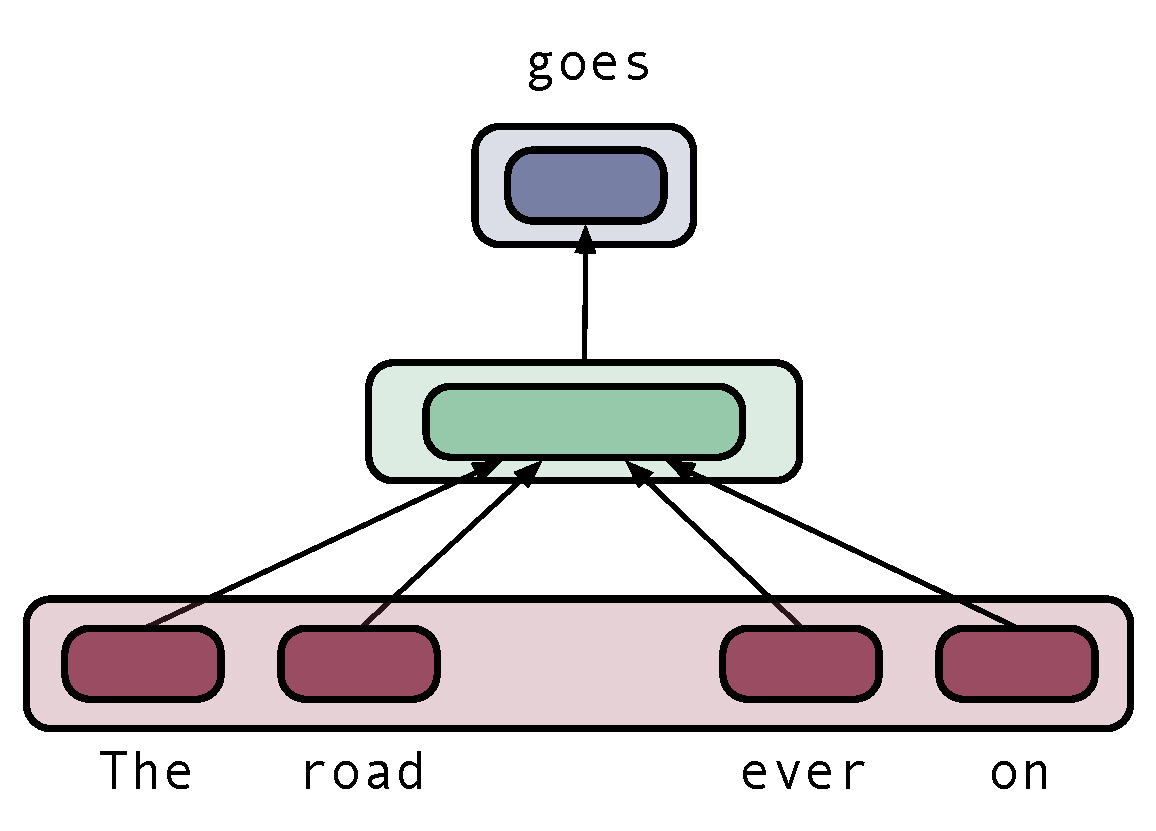
\includegraphics[width=.8\linewidth]{02-background/figs/cbow.pdf}
  \caption{CBOW model}
  \label{bgcbowfig}
\end{subfigure}
\caption{Representation learning architectures proposed by \citet{mikolov2013efficient}. The CBOW model predicts the current word given the context, and the Skipgram model predicts the surrounding words given the current word}
\label{bgsgcbowfig}
\end{figure}
The CBOW model has a projection layer which is shared between all words. This layer averages the input vectors.
Next, using a classifier, the model predicts the word $w_t$ given the context of words surrounding $w_t$ in a fixed sized window: $[w_{t-c}, \ldots, w_{t+c}]$. The objective of the CBOW model is to maximize the following average log probability:
\begin{align}
\frac{1}{T} \sum_{t=1}^T \log p(w_{t} \mid w_{t-c}, \ldots, w_{t-1}, w_{t+1}, \ldots, w_{t+c})
\end{align}

\noindent where $T$ is the length of the sequence of training words and $c$ is the context window size.
The Skipgram model is similar to CBOW, but instead of predicting $w_t$, the model predicts the words within a fixed range surrounding $w_t$.
The objective of the Skipgram model is to maximize the following average log probability:
\begin{align}
\frac{1}{T} \sum_{t=1}^T \sum_{\substack{-c \le j \le c \\ j \ne 0}} \log p(w_{t+j} \mid w_{t})
\end{align}

\noindent where $T$ is the length of the sequence of training words.
Note that in both CBOW and Skipgram models, the context window includes both the past and the future.

\citet{pennington2014glove} combined count-based matrix factorization and context-based Skipgram model together.
The intuition is that meaning of words can be captured by the ratios of co-occurrence probabilities.
They proposed a weighted least squares model that trains on global word co-occurrence counts. 
They showed that the vector space learned from this model captures meaningful vector space substructures.
While some syntactic and semantic features in language are captured by these word embeddings \citep{mikolov-etal-2013-linguistic}, the dimensions are often not interpretable. 

These models utilize surrounding words as context.
However, word representations can capture different phenomena if the definition of context is different. 
\citet{levy2014dependency} proposed to use dependency-based contexts, extracted from dependency parse-trees. 
They observed that these embeddings are less topical and exhibit more functional similarity than the original Skipgram embeddings.

Static embeddings for the most part learn a static matrix of embeddings for each word type and ignore capturing some nuances of language such as ambiguity. 
In Chapter~\ref{chapter:research-01}, we address this issue by exploring document topics and learning multiple embeddings per word type to capture polysemy. 

\subsection{Dynamic embeddings} 

Static models generate out-of-context embeddings for word types and are simple and efficient to train and use. 
However, learning meaningful word representations has recently been elevated beyond this paradigm. 
Rather than learning static representations for word types, these models learn \textit{dynamic} vectors for word instances in context using language modeling objectives. 
We denote this kind of embeddings as dynamic because instead of a static matrix of embeddings, they are obtained through the hidden states of a language model given the context.

\citet{peters-etal-2018-deep} proposed to use a bidirectional recurrent neural network to extract context-dependent representations.
The learning objective is to predict the next word in a sequence, given the previous context words. 
\citet{devlin-etal-2019-bert} use a transformer architecture and define two new objectives for training: \textit{masked language modeling}, and \textit{next sentence prediction}.
During masked language modeling, they mask a randomly selected word in a sentence, and the model has to predict that word given the context.
The second objective gets two input sentences and predicts whether the second sentence is indeed the next sentence.
The contextualized word embeddings are successful at downstream NLP tasks such as question answering and textual entailment \citep{zhang2019semanticsaware,garg2019tanda,Lan2020ALBERT:,mandar2020}.

While word vectors in neural translation models can be initialized with these static or dynamic word representations, they are often initialized randomly \citep{wu2016google}. 
One reason can be that with large-scale parallel data, these initial word representations will be forgotten during the training of the NMT model. 
\citet{qi-etal-2018-pre} showed that for low-resource language pairs and when languages are more similar, pre-trained embeddings can be effective.
\citet{lewis2019bart} recently proposed a denoising autoencoder model named BART for pretraining sequence-to-sequence models. 
They corrupt text with an arbitrary noising function and learn a model to reconstruct the original text.
BART is effective when fine-tuned for text generation and translation but also works well for comprehension tasks.
The research presented in this thesis mostly predates the work mentioned in this section.
We use \textit{static} embeddings in Chapter~\ref{chapter:research-01} where we investigate the effect of having more than one representation per word type. 
As for the chapters on machine translation, we consider the most widespread setup where embeddings are initialized randomly before training on the parallel data.